\section{Overview}

\begin{figure}[tbhp]
  \begin{center}
    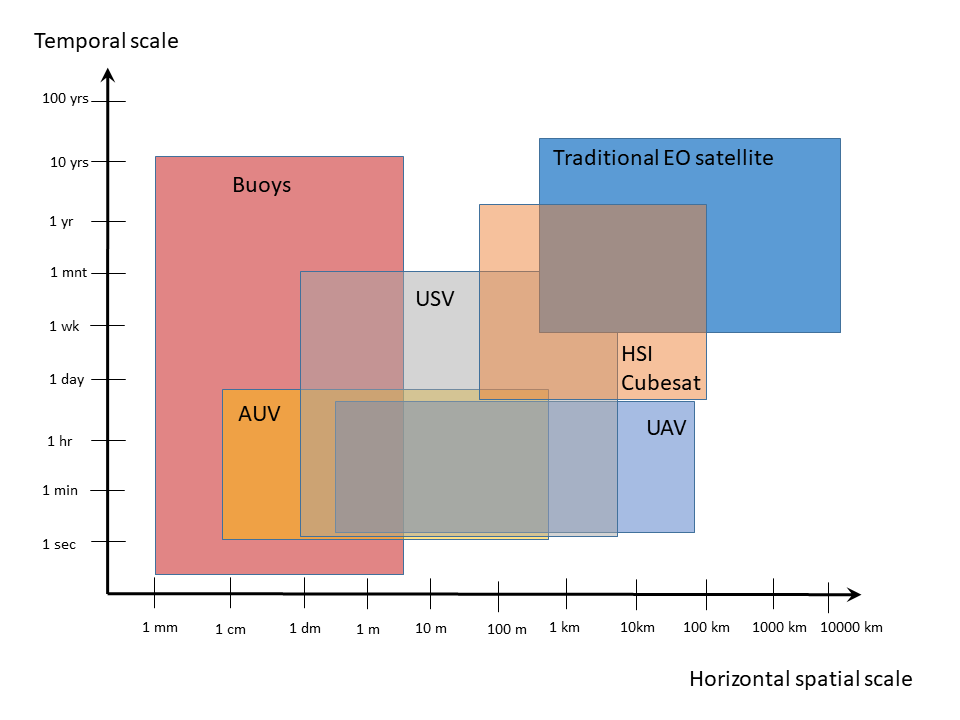
\includegraphics[width=90mm,angle=0]{figs/scales.png}
    \caption{Mapping of capabilities of various sensor platforms used for ocean color.}
    \label{fig:scales}
\end{center}
\end{figure}

Figure \ref{fig:scales} summarizes the capabilities of the different
agents in an autonomous marine observation system, such as the one
illustrated in Figure \ref{fig:overview}, dedicated for our intended
application to ocean color observations with the HSI.  

\begin{table*}[htbp]
	\centering
			\caption{\hypso Mission Overview}
		\begin{tabular}{|l|p{12cm}|}
			\hline
			\textbf{General}	&			\textbf{Definition} 			\\ 
			\hline
		  Objective       &   Ocean color \\
			Subjects & Norway, Greenland, Svalbard, Barents Sea, Baltic, Chiloe, Cape Point, Antarctica, Monterey Bay, Azores \\
			Target Location (baseline) & Lat: 63.867608 $^{\circ}$, Lon: 8.663644 $^{\circ}$ (Fr{\o}ya, Norway) \\
			Target area & 70 km $\times$ 70 km$^2$\\
			\hline
			\textbf{Orbit}	&						\\ 
			\hline
			Type      & Syn-Synchronous \\
      Altitude        &        500 km \\
			Repeat Cycle & 7 days \\
			Launch & 10:00 AM LTAN in Q2 2020 \\
		  \hline
			\textbf{Payload}	&			 			\\ 
			\hline
			Type       &  Pushbroom Hyperspectral Imager \\
			Spectral Range & 400-800 nm \\
			Spectral Resolution & 3.34-10 nm \\
			Max FPS & 39.56 \\
			ADC resolution & 12 bit \\
			Spatial resolution &  693.65 m \\
			Swath Width & 70.32 km \\
      Ground Sampling Distance & $<$39 m \\
			Max raw SNR & 198.73 \\
			Max effective SNR & 486.78 \\
			\hline
			\textbf{S/C Bus} & \\
			\hline
			Size        &         6U \\
	    Energy     &         94 Wh \\
			Mass     &         	6.8 kg \\
			Secondary payloads & RGB camera, SDR \\
			\hline
			\textbf{Autonomy}	&			 			\\ 
			\hline
			Data Processing & On-board compression, geometric, radiometric, spectral and spatial processing \\
			Downlinked Data Products & Level 1A and Operational data (L4: spectral signatures+map coordinates) \\
			Autonomy & Uplink and downlink to Ground Station, uploaded scheduling and tasks determined by mission control \\
		  \hline
			\textbf{Communications} &			 			\\ 
			\hline
			Radios      &  S-band (uplink/downlink), UHF (back-up and commissioning) \\
			Ground Stations & NTNU Trondheim, KSAT Svalbard \& Troms{\o} \\
			\hline
		\end{tabular}
	  \label{tab:mission_concept}
\end{table*}

The right end of the horizontal spatial scale axis defines the spatial
coverage of the HSI sensor system (defined as
$\sqrt( range \times swath)$), while the left end defines the smallest
spatial scales that can be captured by a HSI sensor on the
platform. The upper end of the temporal capability defines the
endurance of the platform, while the lower end illustrates the revisit
time or fastest temporal scales that can be observed. It should be
noted that the endurance of UAVs, USVs and AUVs may typically be
easily extended by fast re-launch after re-fueling. We also remark
that there are other important dimensions beyond the temporal and
horizontal spatial scales that also characterize the differences
between platforms. One important dimension is related to the maximum
speed of UAVs, USVs and AUVs implying that high temporal and spatial
resolution can only be achieved within limited parts of areas
that are within their range. 

This means that these type of vehicles will need adaptive sampling and
be guided towards ``interesting'' parts of the target area where it can be
expected to make informative observations, \cite{Bel93}. Other
important dimensions are related to weather sensitivities, payload
weight limitations, and operational complexity. The figure clearly
illustrates the complementary capabilities of the different sensor
platforms, and shows the scope for a coordinated observation system
that exploits the advantages of each platform type.

Based on Figure \ref{fig:scales}, a \sml capability is generally
differentiated from exquisite and monolithic optical EO satellites 
by having a better temporal, spectral and spatial resolution, but
within a much smaller area and shorter lifetime. It is clear that a
constellation with multiple HSI \sml will extend the capability in
all dimensions compared to a single \smle. We also observe that a HSI
\sml is a useful and complementary platform to AUVs, USVs, UAVs and
buoys/drifters in particular given the limited mobility and speed of
the mentioned platforms. In particular, the capabilities covered by
\smle, UAV and USV are very well aligned by with requirements for
observing highly transient phytoplankton blooms \cite{Dic05}.

In order to achieve high spectral, spatial and temporal resolution of
a HSI in a \sml system with low cost and low weight, our \hypso design
assumes that the observation target area is limited to a small
number of patches of the Earth (possibly only one), typically at least of size
30 km$\times$30 km, cf. Figure \ref{fig:scales}. We emphasize that our
system objective is not to map the entire Earth, but a tiny fraction
corresponding to our specific target area(s) of interest. This enables
the use of an imaging system with a relatively narrow FoV corresponding to a swath width of 70 km. By accurate attitude
control and slewing motion, the push-broom HSI will sweep over this
small area as illustrated in Figure \ref{fig:conops1}.

\begin{figure*}[tbhp]
  \begin{center}
    \includegraphics[width=150mm,angle=0]{figs/conops1.png}
    \caption{Concept of operations for \hypsoe in retrograde near-polar orbit.}
    \label{fig:conops1}
\end{center}
\end{figure*}

The different phases in the operation of the \hypso are shown overall in Fig. \ref{fig:conops1} and are as follows:

\begin{enumerate}

\item Cruise: \hypso will spend most of its time in Cruise
  mode, where it primarily harvests solar energy.

\item Upload: \hypso is scheduled to initialize operations before
  it passes the target area. In preparation for the observations, 
	if available, a nearby ground control station (GCS) uploads tasks and updates to the mission planning \& scheduling of \hypso. This may include changes in target area size and location, atmospheric variables, observed solar zenith angle, commanded viewing angle, desired ground sampling distance, camera settings, and data from observations made by other assets
  (UAVs, USVs, etc.) to be used for radiometric and spectral calibration. \footnote{For example, a USV or UAV
    might tactically emit gas to form an artificial cloud of the size
    of at least one pixel at a suitable location and time such that it
    can be used to calibrate the satellite's HSI in space, time and
    spectrum.}

\item Preparations: \hypso activates mission-specific attitude controller in order to pointing the sensing axis towards the target before actuation of the spacecraft to move in opposite direction of in-orbit track.

\item Start observation: \hypso starts recording line scans from
  the HSI while under slewing
  motion. It scans slowly over the target area in order to
  maximize the spatial resolution along the surface and achieving GSD less than the payload's raw spatial resolution. With near-real-time geo-referenced data input, the images are fused in deconvolution filter or super-resolution/image fusion techniques.  \hypso stores the consecutive data which later undergo 
	data analysis and compression algorithms onboard.

\item End observation and data processing: After the target area is
  scanned, \hypso starts geometric, radiometric, spectral and spatio-temporal processing and
	automated analysis of the data cube in search of positive signatures that match a-priori reference data or unexpected signatures that are new to the model.

\item Download: Depending on the location of the next GCS, \hypso might directly downlink the
  results of its tasks, or go to idle-mode before scheduled to wake up again and initialize for communications at a later stage.

\item Sleep: \hypso goes back to Cruise mode where it harvests solar energy before entering eclipse.

\item Data processing: Ground will either process L1A data or operational data (L4) on ground. Verification, control and validation of the data and onboard processing chain is necessary here.
	
\item Other: imaging operations of other target areas i.e. larger targets and image size(s), other data products, ground-space vicarious calibration, and on-orbit calibration.
\end{enumerate}

% \begin{figure}[tbhp]
%   \begin{center}
%     \includegraphics[width=85mm,angle=0]{figs/concept2x.png}
%     \caption{Conceptual overview: Several passes of the cube-satellite
%       from north to south in polar orbit near the target area.} 
%     \label{fig:con2}
%   \end{center}
% \end{figure}
%\begin{figure*}[tbhp]
  %\begin{center}
%%    \includegraphics[width=160mm,angle=0]{figs/concept3.png}
    %\includegraphics[scale=0.03]{figs/concept3.jpg}
    %\caption{Conceptual overview, including also aerial and surface
      %assets, as well as ground control and operations center.} 
    %\label{fig:con3}
  %\end{center}
%\end{figure*}


%The \sml will travel from south to north in a
%sun synchronous orbit (retrograde) at good lighting conditions. This operation is not limited to be at any other high-inclination 
%Low-Earth-Orbit (LEO) configurations that could meet the mission requirements. 
%Given that the orbit is retrograde and since the northern GCS is within reach during this pass, the
%\sml is able to downlink the data results promptly after observations in pass $N$. In pass $N+1$ the \sml wakes up
%to receive telemetry and commands from the southern GCS before making
%observations when passing the next target area. Slightly later
%the data results are downloaded at the northern GCS before the \sml
%goes to harvesting mode. In passes before and after direct overhead imaging, the \sml nominally harvests solar energy, but may also observe the same target at higher incidence angles with several revisit times. An overview of current iteration on mission design and spacecraft systems is given in Table \ref{tab:mission_overview}.